\documentclass[12pt]{article}

\usepackage{amsmath}
\usepackage{amssymb}
\usepackage[a4paper, margin=1.5in]{geometry}
\usepackage{graphicx}
\usepackage{booktabs}
\usepackage{dsfont}
\usepackage{setspace}

\usepackage[T1]{fontenc}
\usepackage{helvet}
\renewcommand{\familydefault}{\sfdefault}


\title{Dissertation on EV Adoption and Policy Incentives}
\author{Runbin Wang \\ University College London - MSc Economics\\ }
\date{\today}

\begin{document}
\onehalfspacing
\maketitle
\section{Abstract}

\newpage

\tableofcontents

\newpage  


\section{Introduction}

Electric vehicles (EVs) have emerged as a pivotal technology in the global transition towards sustainable transportation. 
EVs can be devided into battery electric vehicles (BEVs) and plug-in hybrid electric vehicles (PHEVs), both of which offer significant advantages over traditional internal combustion engine (ICE) vehicles, 
including reduced greenhouse gas emissions, lower operating costs, and improved energy efficiency.
Governments worldwide have implemented a range of incentives to accelerate EV uptake, such as direct purchase subsidies, tax rebates, and exemptions from registration fees. 
In addition, indirect incentives such as investments in Electric Vehicle Supply Equipment (EVSE), preferential access to urban zones, 
and public awareness campaigns have played a significant role in shaping consumer behavior. 
As EV technology continues to evolve, policy incentives remain a critical lever for driving adoption and achieving environmental objectives. 
As one of the greatest carbon emitters, China committed to carbon neutrality by 2030 and has put significant policy power into environmental policies. 
China remains the world's largest automobile market, the transportation sector, as a traditional carbon-intensive industry, presents as one of the greatest challenges yet a great opportunity to decarbonization. 
China's average annual growth rate hits approximately 15\% in automobile base since 1990, the momentum in the traditional automobile industry makes the transition toward sustainable transport especially difficult. 
Therefore, the question of how to efficiently incentivize EV adoption closely links to environmental policy frameworks, which aim to mitigate greenhouse gas emissions and reduce urban air pollution. 
    
The unique nature of the two-sided market between EVs and charging stations presents a special opportunity for policy design, 
leveraging the presence of feedback effects caused by the indirect network externalities between the two sides. 
That is, the demand for EVs is influenced by the availability of EVSE for reasons like range anxiety and usage costs, while the expansion of charging networks is driven by the number of EVs on the road.
Global successes with EV penetration have demonstrated the need for government intervention, but leaving the matter of efficiency underexplored. 
EV policies have been pivotal to the net-zero target of China, where a wide-range of policies have been entering, substituting and phasing-out in a frequent basis, 
allowing for many additional policy questions to be answered by evaluating the rich set of policy mix.
Therefore, this study structurally models vehicle purchase decisions and charging infrastructure provision in China, identifying the indirect network effects between EVs demand and charging network,
and answers policy questions and evaluates policy efficiency in incentivizing EV adoption and charging network expansion.

To my knowledge, structural estimations in the Chinese automobile industry that incorporates indirect network effects are very limited. 
By establishing structural model for both sides of the market, I can recover key estimates such as responsivenss of purchase and EVSE provision to policies and price elasticities,
which allows me to examine the network effects and conduct counterfactuals in answering different policy questions.  
Motivated by the proposed 'non-neutrality' of subsidies by Springel (2021), this study empirically examines this pattern and its implications for policy design in the context of the Chinese market.
The Chinese market leads the world in both sides of the market, with its sales taking up 60\% of global EV sales in 2023 and its EVSE infrastructure network largest in scale (International Energy Agency, 2025).
More specifically, the key model parameters determines which is more efficient, subsidizing purchases of EVs or charging infrastructure entry.
The answer to this question comes down to an empirical examination of the interaction between EVs and charging stations, in which several factors come into play.
First, the importance of consumer valuation in charging network in relative to other factors affecting EV adoption determines the overall effectiveness of charging subsidies, 
and similar arguments hold for the impact of the EVSE subsidies. Additionally, the substitutional patterns of EV and ICE models, substitutions within EVs, 
and the magnitude of feedback effects, all together change the effectiveness of price subsidies. 

In order to answer the research questions, I first build a structural model of vehicle demand based on random utility maximization. 
I adopted a discrete choice framework, specifically, a nested logit model that describes the purchase decision process of consumers in the automobile market,
incorporating relevance of charging infrastructure availability to consumer preferences and allowing for flexible substitutional patterns. 
Accounting the for the simultaneous nature of the two-sided market, I also build a supply-side model of EVSE provision, 
which describes the entry decision of EVSE providers in response to the number of EVs on the road and the incentives provided by the government.
The two models helps recovering key primatives that facilitates the quantification of indirect network effects and counterfactual analyses,
namely the semi-elasticities of EV demand with respect to charging infrastructure availability, that of EVSE provision with respect to EV base and incentives, and the price elasticities.
A key challenge in this context is the potential endogeneity of the variables involved, due to prices, EV demands and EVSE provisions all being equilibrium outcomes,
and endogeneity regarding the simultaneity of the two-sided market are addressed by using instrumental variables.

Results from estimations confirm the existence of indirect network effects in both sides of market. 
In particular, with estimated a negative price estimate, vehicle models act as substitutes without network effects. 
In terms of the two-sidedness, estimation returned positive semi-elasticities for both directions, but the indirect network effects on elasticities still show some degree of heterogeneity.
Impacts on price elasticities exhibits varying magnitudes, even directions across markets. 
Change in price structure under indirect network effects may lead to complementarity between EV models in some markets, whereas in others, it may reinforce substitution effects.
Complementarity comes from the feedback loop between EV adoption and charging infrastructure expansion, where decreased prices, although leading to substitutions into that model from others,
may increase total EV base, which in turn leads to expanded charging network and stronger demands for all EV models.

I then conduct two sets of counterfactuals, with the first set comparing the impact of different policy instruments to EV and EVSE diffusion,
measured from a no-incentive baseline scenario. The results show that the current combination of incentives on both sides of the market, together yields 4.7\% more EV sales and 3.3\% more charging piles.
Each additional million CNY spent on the policy mix resulted in 8.29 more EV sales and 0.8 more charging piles.
Comparison between demand-side instruments indicates that a uniform purchase subsidy is the most efficient overall.
As for EVSE, demand-side incentives do exhibit moderate level of spillovers to charging stations, but direct EVSE incentives are more than three-times in efficiency in promoting EVSE deployment.
However, the subsidizing EVSE exhibits limited influence on EV adoption, with only approximately 15\% effectiveness as compared to direct incentives on EV prices.
The second set of counterfactuals further investigates the marginal efficiency of purchase subsidies and EVSE incentives.
The result shows limited diminishing returns and supports the use of purchase subsidies for EV diffusion,
while suggesting the possibility of an over-developed charging infrastructure network in China that resulted in minimal feedback effects.
The estimation results provide insights for future policy design, suggesting for targeted policy choices instead of adopting inefficient policy mix.

From hereafter, this paper is structured as follows: first, relevant background information on market, literature, and data are introduced in sections 3, 4, and 5 respectively;
Section 6 and 7 then discuss the modelling details and empirical strategies for estimations. Finally, the results are presented and used for counterfactual analyses in sections 8 and 9,
and section 10 concludes.

\section{Industrial Background and Policy}
    \subsection{EV market}
To achieve the announced policy objective of hitting 60\% EV market share by 2030, Chinese government has implemented a range of policies to promote EV adoption, 
including direct monetary incentives, indirect policies favouring EV usage in transport, and the recent shift of focus onto charging infrastructure. 
The Chinese EV market has experienced a rapid expansion period over the last decade, and various incentives in the form of both central and disaggregated policies have contributed to the process. 
Back in 2009, the Chinese government first initiated the experimental policy initiative of "1,000 EVs in 10 cities", aiming at introducing new energy vehicles at 10 cities per year. 
To initialize EV adoption, the replacement over traditional ICE cars originated from public transports, taxi, and other government-led fields. 
However, EV penetration was unsuccessful during earlier stages due to immature production technology, lack of scale and insufficient support from infrastructures. 
Within the same period, monetary incentives were also introduced on both supply and demand side in the form of cost rebates and purchase subsidies. 
In 2014, a uniform tax exemption was placed for on all purchases of BEVs and PHEVs. 
In the meantime, local governments following central guidelines, began to initiate indirect policies favouring EVs over traditional ICE vehicles. 
Typical examples were travel restrictions that EVs were exempted from, parking previleges, and additional registration quota for EVs.
With the strong incentives from the Chinese government, complemented with various local restrictions on the ICE vehicles, 
the displacement of ICE vehicles by EVs has been rapid, as shown in Figure 1 taking Shanghai as an example. 

\begin{figure}[htbp]
    \centering
    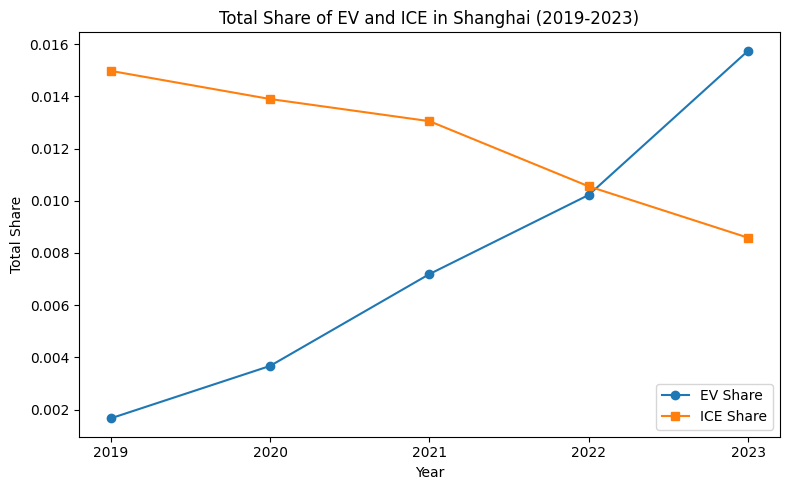
\includegraphics[width=0.7\textwidth]{GraphsTables/total_shares_ev_ice_shanghai.png}
    \caption{EV and ICE Market Shares in Shanghai (2019-2023)}
    \label{fig:total_shares_ev_ice_shanghai}
\end{figure} 

However, the explosive rise of EV market share had a strong reliance on intense monetary incentives, as a result, subsidy frauds also came as a side effect. 
As a result, the attention gradually shifted from direct to indirect policies, among which infrastructure supply was a key target due to the unique two-sided market feature of EV. 
From 2017, direct purchase subsidies started phasing out, substituted by construction cost rebate and operational subsidies for charging infrastructures. 
In addition, the 'Dual Credit Policy' published in 2017 effectively ensured a minimum share for EV sales from the supply side, also resulted in a large scale entry of traditional ICE automobile players into EV production. 
In consequence, competition intensified accompanied with a rapid increase in the number of models available.
Following the expansion of the technology frontier which reduced product differentiation in low-end models, aggressive pricing behaviours were widely adopted in response to the increase in price sensitivity.

In the period of 2019-2023, after the complete phasing-out of uniform purchase subsidies, attribute-based subsidies and tax exemptions were the only major central incentives remaining. 
Range-based subsidies and infrastructure deployment requirements were introduced to lead the market towards solving range-anxiety associated with EVs. 
Throughout the period, range-based subsidies continued to phase-out from low to high range categories following previously determined schedules, creating exogenous time variations for policy evaluations. 
Table~\ref{tab:subsidies} shows the ramp-down schedule of range-based subsidy for BEVs and PHEVs.

\begin{table}[!htbp]
\centering
\caption{Range-Based Subsidy Schedule by Year (10,000 CNY)}
\label{tab:subsidies}
\begin{tabular}{@{}lcccc@{}}
\toprule
Year & \multicolumn{1}{c}{PHEV} & \multicolumn{2}{c}{BEV} & \multicolumn{1}{c}{} \\
\cmidrule(lr){2-2} \cmidrule(lr){3-4}
Range & $R \geq 50$ & $300 \geq R \geq 250$ & $400 \geq R \geq 300$ & $R \geq 400$ \\
\midrule
2019 & 1.00 & 1.80 & 1.80 & 2.50 \\
2020 & 0.85 & 0.00 & 1.62 & 2.225 \\
2021 & 0.68 & 0.00 & 1.30 & 1.80 \\
2022 & 0.48 & 0.00 & 0.91 & 1.26 \\
2023 & 0.00 & 0.00 & 0.00 & 0.00 \\
\bottomrule
\end{tabular}
\end{table}

    \subsection{EVSE market}
In comparison to the EV market, the EVSE market is much more concentrated with top players dominating market shares.
In 2023, out of the total 2.7 million public charging piles, the top 5 EVSE providers occupied over 62\% of the market share and 81\% of total charging power output.
Following the phasing-out in EV purchase subsidies, the focus of incentives has shifted towards charging infrastructure, targeting EV-piles ratio.

\begin{figure}[htbp]
    \centering
    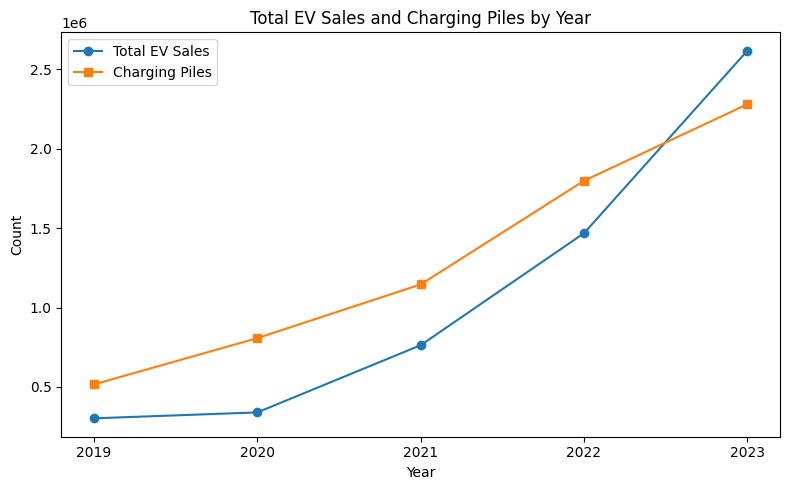
\includegraphics[width=0.7\textwidth]{GraphsTables/total_ev_charging_trend.png}
    \caption{EV Stock and Charging Piles Stock in China (2019-2023)}
    \label{fig:EV_charging}
\end{figure}


\section{literature Review}
This study primarily relates to the following three strands of literature. Firstly, this study closely relates to the mature literature on differentiated product demand estimation, 
in which the automobile market has been specifically focused on with a variety of directions for extensions. 
Following the foundational work of MacFadden (1977), the strucutral approach of logit discrete choice has been widely adopted for the demand-supply style problems. 
To allow for more realistic substitution patterns and promptly deal with dimensionality problems, 
variants in the model such as the nested logit model, the principles-of-differentiation general extreme-value (PD-GEV) model in Bresnahan et al. (1997), 
and the adopted approach in this paper of random-coefficient discrete choice model in Berry et al. (1995). 
Following the seminal works of Bresnahan (1987), Berry et al. (1995), and Petrin (2002), I apply the standard structural modelling techniques to the automobile industry, 
in order to recover flexible substitution patterns and facilitate counterfactual policy evaluations. Although automobile demand estimation has been thoroughly discussed in the past three decades, 
the focus on EV is relatively fresh within the literature. Li et al. (2017) began with a stylized model to evaluate the effectiveness of EV and infrastructure incentives in the U.S. market. 
They found that charging station subsidies of equal sizes are twice as effective for EV adoption that purchase incentives. 
Springel (2021) asked a similar question in the Norwesian market, but implemented a structural demand-supply equilibrium setup and estimated a random coefficient model under the influence of indirect network externality of charging stations, 
which then faciliates a range of policy counterfactuals. Li (2023) considered again the U.S. automobile market and EV adoption using a BLP-style model, 
but introduced incompatible charging standards to the supply side and focused primarily on the impact of a standardization policy for EV penetration. 
Remmy (2024) expanded the strucutral model by endogenizing supply-side decision on range of EVs and explored firms', in addition to consumers', responses to incentive schemes in Germany. 
Finally, Heid et al. (2024) enriched the modelling further by bringing in electricity market to form a joint-equilibrium model, endogenizing charging timing on the demand side, and further discussed the issue of pass-through in incentives. 
As for studies on the Chinese automobile industry, Jia et al. (2023) studied the impact of attribute-based incentives to EV adoption building on a structural demand model. 
They found that But they focus primarily on the strand of endogenous product attributes and abstracted away from the supply-side decision on charging station entry. 
To the best of my knowledge, there is yet a comprehensive study of the Chinese EV market that incorporates indirect network effects.\\

Secondly, the interaction between EV and charging station presents a typical example of a two-sided market, in which the presence of indirect network effect would generally alter policy implications significantly. 
The literature on indirect network effect traces back to the earlier theoretical works such as Katz and Shapiro (1985), and Farrel and Saloner (1985),
which was then extended to a formal two-sided 'platform' framework by studies such as Rochet and Tirole (2003), Wright (2004), and Armstrong (2006). 
As shown by Wright (2004), in applying tools to evaluate competition and industrial structures, neglecting the two-sidedness of a market can lead to serious mistakes in results.
The theories predict a positive feedback loop that increased volume of one side would increase the value of the other side, which in reverse further benefits the former side.
In terms of the EV market, the network effects is generated from the interaction between EVs and charging stations, 
where a larger stock of EVs would increase the profitability for EVSE providers and give rise to expanding charging network, which in turn increases the convenience of owning an EV.
However, the network effects adds complementarity to the traditional force of competition that makes EVs substitutes, leaving the net effect ambiguous.
More recent studies such as Clements and Ohashi (2005) in video games market, Filistrucchi et al. (2012) in newspaper market, 
and Reshef (2023) in online takeout platform, have identified material conclusions of how positive indirect network alters competition.
As for the EV literature, following Li et al. (2017) and Springel (2021), recent studies have all taken indirect network effect into account when considering EV penetration.
This study specifically considers how would the presence of indirect network effect alters EV policy effectiveness in the Chinese market. \\

Lastly, this paper contributes to the understanding of policy impacts on EV adoption and environmental implications, which is made different by the consideration of indirect network effects. 
Subsidies in promoting diffusion of clean-energy technologies have shown to be an effective environmental policy instrument (Acemoglu et al., 2016).
The growing literature of EV adoption and environmental policy has studied cases of various developed economies, 
such as in Norway (Springel, 2021; van Dijk et al., 2022; Koch et al., 2022), the US (Holland et al., 2016; Li et al., 2017; Li, 2023), Germany (Heid et al., 2024; Remmy, 2024;), and in China (Guo and Xiao, 2023; Barwick et al., 2024; Zhu et al., 2024).
One strand of literature adopts comprehensive econometric models to recover key parameters, then run policy counterfactual analysis in order to evaluate a variety of policy instruments.
Studies have examined a variety of approaches of policy interventions in promoting EV penetration, including demand-side targets like direct purchase subsidies (Guo and Xiao, 2023) 
and attribute-based subsidies (Jia et al., 2023; Barwick et al., 2024), also in supply-side targets like EVSE subsidies (Li et al., 2017; Springel, 2021; Zhu et al., 2024) and charging standards (Li, 2023).
Additionally, a subset of literature approaches EV penetration from a technology diffusion point of view, focusing on multiple equilibriums and critical mass for EV and charging infrastructures to self-sustain (Zhou and Li, 2018; Koch et al., 2021; van Dijk et al., 2022).
In terms of measuring EV policy implications, studies such as Holland et al. (2016), Guo and Xiao (2023), Heid et al. (2024), and Barwick et al. (2024),
have documented heterogeneous conclusions on welfare effects, some supports current incentive structures while others suggest for a ramp-down of subsidies. 


\section{Data}
The data I use is combiled from a variety of sources, including a commercial source that aggregated registry data from the Chinese Association of Automobile Manufacturers (CAAM), 
indiative price and range data from the Minstry of Industry and Information Technology (MIIT), 
charging piles stock data from the China Electric Vehicel Charging Infrastcture Promotion Alliance (EVCIPA), 
the province-level demographic data National Bureau of Statistics (NBS), and supplementary information on a wide-range of government incentives at different levels.

The primary data set is the sales data where each entry contains the number of sales for a particular model within a province in a given year during 2019-2023, 
it also contains brand, fuel-type and two supplementary product characteristics of each model: mass and power. 
This data set is over all types of private cars, consisting ICE cars and EVs that can be further divided into BEVs and PHEVs. 
The data set was purchased from a commercial source that aggregated micro data of Compulsory Traffic Accident Liability Insurance (CTALI) maintained by the CAAM.
It is common practice to use this measure as proxy for car purchases in the Chinese market, as CTALI registed cars are the ones actually in-use. 
The number of models appears to vary across years and the availability of some are not uniform across provinces. 
I define a market as a province-year pair, and a the unit of observation at the model-market level.
The data set consists of 31 provinces over a 5-years interval with varying models existing in different markets, giving me a total number of 25260 observations. 
This sample size is significant compares to other studies due to the large geographic dimension and uniquely rich diversification in the Chinese automobile market, supported by its market base.

The second data set I built by combiling registration information on EV models, Manufacturer Suggested Retail Price (MSRP) and range published by the MITT, 
and I use the midpoint of the MSRP interval as a proxy for the market price. The regulation in the Chinese market sets a price floor for the manufacturers, 
thus the use of MSRP can be seen as reasonable proxy for transaction prices. 
The data set also contains the range and battery capacity of each model, which I use to match models to subsidy schedules and as observed product characteristics.

I also obtain the charging piles stock at the province-year level from 2018-2023.
Different to previous studies that used the number of charging stations which is not readily available for the Chinese market, 
I use the number of charging piles as the measure of charging infrastructure.
This measure is directly relevant to consumers' charging decisions while still fits into the commonly assumed modelling framework. 
As previously introduced, EVSE industry in China is highly concentrated with a partially-regulated nature, meaning that charging points are largely standardized.
Additionally, as the incentives on charging infrastructures are primarily in the unit of charging piles, it is more natural to use the number of charging piles as the measure of charging infrastructure.

Lastly, I combile from a wide range of Chinese government sources information on central and local policies as well as other statistics.
Due to limited scope of this paper, I focus on central policies, accompanied by a small set of province-level polilcies that are easy to quantify and large in scale. 
Control measures such as local demographics and transportation measures are also included for the purpose of controls, determining market-sizes, and construction of instrumental variables.
I follow common practice to use number of households in a market as total market size.

\begin{table}[htbp]
\centering
\caption{Descriptive Statistics: Combined Demand and Supply Data}
\label{tab:combined_descriptive_stats}
\resizebox{\textwidth}{!}{
\begin{tabular}{lrrrrr}
\toprule
Variable & Count & Mean & Std Dev & Min & Max \\
\midrule
\textbf{Demand Variables} & & & & & \\
Sales & 33,545 & 854 & 2,500 & 1 & 121,388 \\
Price (10k ¥) & 33,545 & 19.8 & 13.4 & 3.4 & 141.6 \\
Net Price (10k ¥) & 33,545 & 17.7 & 12.2 & 1.8 & 129.0 \\
Range (km) & 33,545 & 326 & 177 & 52 & 742 \\
Power (kW) & 33,545 & 124 & 43 & 0.9 & 814 \\
Battery Capacity (kWh) & 33,545 & 587 & 838 & 12 & 2,743 \\
Charging Piles & 33,545 & 50,045 & 68,287 & 18 & 502,968 \\
\midrule
\textbf{Supply Variables} & & & & & \\
Charging Piles & 155 & 42,202 & 60,769 & 18 & 502,968 \\
EV Stock & 155 & 295,838 & 376,660 & 733 & 2,338,897 \\
Fixed Subsidy (¥/kW) & 155 & 25.7 & 86.5 & 0.0 & 400.0 \\
Operating Subsidy (¥/kWh) & 155 & 0.03 & 0.10 & 0.00 & 0.55 \\
\bottomrule
\end{tabular}
}
\end{table}


\section{Modelling}
    \subsection{Demand: Vehicle Choice}
    For modelling vehicle demand side, I follow the tradtitional setup of differentiated product demand estimation to use a random utility maximization setup for modelling of discrete choices. 
In particular, assume there re \textit{m = 1,...,M} markets that is defined as a province-year pair within my context of study. Within each of the defined market, the modelling is on individual purchase decisions of \textit{i = 1,...,I\textsubscript{m}} number of potential consumers, 
made over \textit{j = 1,...,J} different vehicle models in the product space. The conditional indirect utility of consumer $i$, $U(x_{jt}, \xi_{jt}, p_{jt}, \tau_i; \theta)$ of consuming product $j$ in market $m$ is specified as a function of both observed and unobserved product characteristics:

\begin{equation}
    u_{ijm} = \beta^{EV} EV_j+ \beta^N \log(N_m) + \beta^N_{EV} (\log(N_m) \times EV_j) + \alpha p_{jm} + x^{K}_{jm} \beta^{K} + \xi_{jm} + \bar{\epsilon}_{ijm}
\end{equation}
$i = 1,...,I_m, \ j = 0,..,J, \ m = 1,...,M,$

where $EV_j$ is an indicator equal to 1 if the model is EV, $N_{m}$ denotes the number of public charging piles in the market, 
$p_{jm}$ denotes the net product price of product $j$ in market $m$, 
$x^{k}_{jt}$ is a $K$-dimensional row vector of observable produt characteristics of product j,
including power, range and battery capacity, where range and battery capacity are set to 0 for non-EVs, 
$\xi_{jm}$ is the unobservable characteristics,
and $\bar{\epsilon}_{ijm}$ is a mean-zero stochastic term representing the remaining idiosyncratic valuation for product $j$. 

Different to earlier studies, I allow for general effect of EVSE availability on all vehicles,
which captures the impact of public infrastructure favouring EVs that put limitations on ICE vehicles,
and the network feedback is measured by the combined effect of $\beta^N$ and $\beta^N_{EV}$.

Additionally, an outside good representing no purchases is defined to have indirect utlity of $u_{i0m} = \bar{\epsilon}_{ijm}$.
Consumer $i$ chooses between the outside good 0 and other $J$ differentiated products in the market and purchases one unit of good $j$ if and only if $u_{ijm} > u_{ikm}$ for all $k \geq 0$ and $k \neq j$. 
As a standard practice notation-wise, I define the mean utility level of product $j$ in market $m$ as:

\begin{equation}
    \delta_{jm} \equiv \beta^{EV} EV_j+ \beta^N \log(N_m) + \beta^N_{EV} (\log(N_m) \times EV_j) + \alpha p_{jm} + x^{K}_{jm} \beta^{K} + \xi_{jm}
\end{equation}

Following the distributional assumptions of the nested logit model, the individual valuation term $\bar{\epsilon}_{ijm}$ can be further decomposed as:

\begin{equation}
    \bar{\epsilon}_{ijm} = \zeta_{igm} + (1 - \rho) \epsilon_{ijm}
\end{equation}

Where $\zeta_{igm}$ is a group-common term of group $g = 0,...,G$, and an i.i.d individual valuation shock $(1 - \rho) \epsilon_{ijm}$. Here, $0 \leq \rho \leq 1$ is the nesting parameter approximates for the degree of preference correlation between products of the same group. 
Following the interpretation of Berry (1994), the group-common term $\zeta_{igm}$ can be seen as random coefficeints on a set of group-specific dummies $d_{jgm}$ that equals to 1 if $j$ belongs to group $g$.
Summarizing above, consumer $i$'s conditional indrect utility can now be written as:

\begin{equation}
    u_{ijm} = \delta_{jm} + \sum_{g} d_{jgm}\zeta_{jgm} + (1 - \rho) \epsilon_{ijm}
\end{equation}

The nested logit model assumes that the i.i.d shock $\epsilon_{ijm}$ follows a type I extreme value distribution, 
and as shown by Cardell (1997), there exist a unique distribution of $\zeta_{ig}$ that $[\zeta_{ig} + (1-\rho)\epsilon]$ also follows an extreme value distribution. 
The distributional assumptions allow for closed-form solutions for the choice probabilities. I categorize products into three nests: ICE vehicles, BEVs and PHEVs. 
In the spirit of Berry (1994), I write the well-known result of choice probability of choosing product $j$ within group $g$, which equivalent gives the within-group market of product $j$:

\begin{equation}
    s_{j/g} = \frac{e^{\delta_{jm}/(1-\rho)}}{D_g}
\end{equation}

where $D_g$ is the denominator that normalizes the choice probability, defined as:
\begin{equation}
    D_g \equiv \sum_{j \in J_g} e^{\delta_{jm}/(1-\rho)}
\end{equation}

The probability of choosing group $g$ and hence the market share of group $g$ can be expressed as:

\begin{equation}
    s_{g} = \frac{D_g^{(1-\rho)}}{\sum_{g} D_g^{(1-\rho)}}
\end{equation}

Thus, the overall market share of product $j$ in market $m$ reads:
\begin{equation}
    s_{jm} = s_{j/g} s_g = \frac{e^{\delta_{jm}/(1-\rho)}}{D_g^\rho [\sum_{g} D_g^{(1-\rho)}]} 
\end{equation}

Specifically, the outside good as the only product in group 0, with normalizations $\delta_0 \equiv 0$ and $D_0 = 1$, has a market share of:

\begin{equation}
    s_{0m} = \frac{1}{\sum_{g} D_g^{(1-\rho)}}  
\end{equation}

From setting out the model and predicted market share, taking natural logarithms of both sides gives an analyitic linear expression for estimation:

\begin{equation}
    \log(s_{jm}) - \log(s_{0m}) = \delta_{jm}/(1-\rho) - \delta\log(D_g)
\end{equation}

Recalling the definition of $D_g$ and $\delta_{jm}$ gives the final form:

\begin{equation}
    \log(s_{jm}) - \log(s_{0m}) - \rho\log(s_{j/g, m}) = \beta^{EV} EV_j+ \beta^N \log(N_m) + \beta^N_{EV} (\log(N_m) \times EV_j) + \alpha p_{jm} + x^{K}_{jm} \beta^{K} + \xi_{jm}
\end{equation}

The additional term $\rho\log(s_{j/g})$ accounts for the correlation of preferences within groups, which is put to the left of equation indicating its endogeneity as in Conlon and Gortmaker (2020).  

I abstract from car supply modelling in this study due to the limited scope to focus primarily on the primary demand estimation and indirect network effects.
I assume that product characteristics are exogenous to the model, and take implicitly the marginal costs as given by the Nash-Bertrand competition assumption.

    \subsection{Supply: Station Entry}
My specification closely follows that of Springel (2021) and Remmy (2023). Let $h = 1, ..., N_{m}$ denote the set of EVSE providers, and $j = 1,...,J$ denote the set of vehicle models. Assume firms are price-setters and that each firm maximizes profits over a subset $J_f$.
Assuming a standard profit function that is quasi-concave in price, the per-consumer profit function is given as $D_{hm}(p_{hm}, p_{-hm}, N_{m}) (p_{hm} - MC_{hm})$, where the per-consumer demand $D_{hm}$ faced by firm $f$ is given by a function of charging network $N_m$, 
own price $p_{hm}$ and the price of competing firms $p_{-hm}$. Similarly to Springle (2021) and Remmy (2023), I make the following similifying assumptions in the spirit of Gandal, kende, and Rob (2000) and Bresnahan and Reiss (1991): 
    1. Symmetric per-consumer demand function;
    2. Constant marginal cost $MC_{hm}$ and sunk cost of entry $F_{hm} $ across all firms $f$ in market $m$;
    3. Each firm earns and equal share of market profit from symmetry.
These assumptions ensures the eixstence of an equilibrium that all firms charge the same price, and the post-entry station profit per-period reads:

\begin{equation}
    \pi_{m} = Q_{m}^{EV} \frac{D(p(N_m)) \phi(N_m)} {N_m}
\end{equation}

where $Q_{m}^{EV}$ is the cumulative EV stock market $m$, $\phi(N_m) \equiv p - MC$ is the equilibrium markup, and $p(N_m)$ is assumed to decrease in $N_m$. For a simpler notation, denote $f(N_m) \equiv \frac{D(p(N_m)) \phi(N_m)} {N_m}$ 

Next, I assume that the entry decision of charging firms is made at the beginning of each period and utilizes a free-entry condition to derive the equilirbium relationship. I also modify notation to replace market $m$ with a province-year pair $pt$ for clarity in timing.
If a firm enters the market in period $t$, it incurs a sunk cost of entry $F_{pt}$, and earns a stream of per-period profits starting next period $(\pi_{pt+1}, \pi_{pt+2}, ...)$. The free-entry condition requires that the expected present value of profits from entering the market is equalized across periods, that is:

\begin{equation}
    -F_{pt} + \sum_{s=1}^{\infty} \frac{\pi_{pt+s}}{(1 + r)^s} = - \frac{F_{pt+1}} {(1 + r)} + \sum_{s=2}^{\infty} \frac{\pi_{pt+s}}{(1 + r)^s}
\end{equation}

Combining the station profit expression with the free-entry condition and taking natural logarithm of both sides, the expression boils down to:

\begin{equation}
    \log(f(N_{pt})) = -\log(\frac{1}{(1 + r)})  - \log Q_{ct}^{EV} + \log(F_{pt} - \frac{1}{1 + r} F_{pt+1})
\end{equation}

Additionally, I leverage the unique feature of the policy structure in China, where province governments perform independent subsidizing polilicies of different forms across the observed period, 
bringing in additional variations to explore policy effectiveness. Functional form of $f(N_{pt})$ is specified as $(bN_{pt})^{-d}$, 
and the sunk cost of entry $F_{pt}$ is a linear function of exogenous cost shifter of fixed and current operating subsidies, 
province demographics which captured by fixed effect $\rho_p$, and time fixed effect $\tau_{t}$. The station entry model is then specified as:

\begin{equation}
    \log(N_{pt}) = \lambda_0 + \lambda_1 \log(Q_{pt}^{EV}) + \lambda_2 FX_{pt} + \lambda_3 OP_{pt} + \lambda_4 \rho_p + \lambda_5 \tau_t + \epsilon_{pt}
\end{equation}

I do not explicitly model the heterogeneous impact of new charging stations on existing stations due to lack of spatial data on stations.
However, as previously discussed, the level of standarization in the Chinese charging industry makes this assumption more reasonable.
Also, I assume the average number of charging piles per station in each market is exogenous after controlling for province fixed effects,
which is based on the fact that charging pile deployment is largely determined by local demand features. 
Therefore, I maintain the charging infrastructure modelling framework and replace station measure with charging piles.


\section{Empirical Strategy}
    \subsection{Identification: Demand}
For the demand side, there are three sources of endogeneity to be dealt with. 
The first being the traditional problem of endogenous prices caused by simultaneity problem of demand and supply.
Following the rich literature on differentiated product demand estimation, I construct insutrments to identify price coefficient.
I construct two sets of instruments, an exogenous cost shifter and a set of differentiation IVs, 
constructed from assumed exogenous product characteristics.

First, following Springel (2021), Barwick et al. (2024), and Remmy (2024), 
I construct the exogenous cost shifter is constructed by interacting mass of a model with steel price index.
Second, I construct a set of differentiation IVs following Gandhi and Houde (2019) using power, range and battery capacity. 
The idea of leveraging exogenous product characteristics proposed in Berry et al. (1995), namely the BLP instruments, tend to cause weak identification in some cases. 
The differentiation IVs qunatifies the level of competition faced by a product through some measures of its position in the product characteristics space.
There are two subsets of instruments, one measures the Euclidean distance of a model's characteristics to other products, 
and the other count the number of local products that are 'close' in characteristics.

\begin{equation}
Z_{jm,\text{Euclidean}}^{k} = \sum_{l \in \mathcal{C}\backslash\{m\}} (D_{m,jl}^{k})^2
\end{equation}

\begin{equation}
Z_{jm,\text{local}}^{k} = \sum_{l \in \mathcal{C}\backslash\{m\}} \mathds{1}\{|D_{m,jl}^{k}| < \textit{sd}(D_{k})\}
\end{equation}

Where $D_{m,jl}^{k}$ is the distance between product $j$ and $l$ in market $m$ in characteristic $k$,
$\textit{sd}(D_k)$ is the standard deviation of product characteristic $k$, and $\mathcal{C}$ is the set of all products in market $m$.
Second, the endogeneity of the charging station network is caused by simultaneously determined equilrbrium between EVs and charging infrastructures.
Similar to Li (2023), I use the lag of charging piles stock as an instrument assuming no dynamics in the shocks to unobservables.
Lastly, the endogeneity of the within-group market share $s_{j/g}$ directly follows from the definition of the nested logit model.
I adopt the traditional approach of using the size of product space of nest $g$ in market $m$ as an instrument.

I argue for exogeneity of these instruments based on the following reasoning. For the cost shifter, 
a commonly known feature of the automobile manufacturers is that frame designs for a model is determined at the beginning of the production cycle (Barwick et al., 2024),
which means that mass is unlikely to be correlated to shocks in unobservables. Additionally, 
based on the assumption of exogenouse product characteristics for car producers, and the large number of competitors in the automobile industry,
the relative position of a product in the characteristics is expected to be exogenous. 
As for the relevance of the instruments, the first stage $R^2$ and $F$ statistics adds validity to the strength of the instruments.

    \subsection{Identification: Supply}
Similarly, the expected feedback effect also introduced endogeneity to the charging station entry model.
The cumulative EV base contains the endogenous part of new sales, which from the demand equation is a function of charging station network,
causing simultaneity problem. An ideal instrument would be the difference in fuel price and electricity price for each market, which exogenously affects the cost of driving ICE vehicles and EVs. 
Unfortunately, similar to the problem of Norway in Springel (2021), China has a uniform gas and electricity price across the country,
and I do not obtain spatial data for gas stations to construct the proposed instrument of gas station density.
I instead use a Bartick-style instrument following Li et al. (2017) and Koch et al. (2021), 
wihch is constructed as the interaction between total length of roads in a market and a national fuel price index.
The idea is that the a national shock in fuel price would affect local cost of driving ICE vehicles differentially, 
and the total road length is a proxy for the level of development of local transportation infrastructure, which impacts the level of fuel consumption.
Another shift-share instrument I use is a sales-weighted average range measure of all available EV models in a market.
This instrument leverage on the fact that the national range-based subsidy schemes itself has multiple steps in range categories,
therefore the higher the range of available models, the more heavily the market is to be subsidized.
Similarly, first stage $R^2$ and $F$ statistics are used to validate relevance of used instruments.


\section{Results}

    \subsection{Demand}
The vehicle demand equation (equation 11) and the charging entry equation (equation 15) are specified as linear IV models and estimated jointly using a two-stage least squares (2SLS).
Results of the demand-side model estimates are displayed in Table~\ref{tab:demand-estimates}. All parameters are of expected sign and statistically significant at the 1\% level.

\begin{table}[!htbp]
\centering
\caption{Demand Model Estimation Results}
\label{tab:demand-estimates}
\begin{tabular}{@{}lc@{}}
\toprule
\multicolumn{2}{c}{{Dependent variable: $\log(\text{shares})$}} \\
\midrule
Price ($\alpha$) & $-0.121^{***}$ \\
& $(0.012)$ \\
Nesting ($\rho$) & $0.811^{***}$ \\
& $(0.115)$ \\
$\log(N_m) \times EV_j$ & $1.188^{***}$ \\
& $(0.066)$ \\
$EV_j$ & $-15.658^{***}$ \\
& $(0.676)$ \\
$\log(N_m)$ & $-0.606^{***}$ \\
& $(0.075)$ \\
Range & $0.004^{***}$ \\
& $(0.000)$ \\
Power & $0.015^{***}$ \\
& $(0.002)$ \\
Battery Capacity & $0.001^{***}$ \\
& $(0.000)$ \\
\midrule
Observations & 33,545 \\
$R^2$ & 0.982 \\
Residual Std. Error & 11.915 (df = 33,537) \\
F Statistic & $72,390.913^{***}$ (df = 8; 33,537) \\
\bottomrule
\multicolumn{2}{@{}l@{}}{\footnotesize \textit{Note:} $^{*}$p$<$0.1; $^{**}$p$<$0.05; $^{***}$p$<$0.01} \\
\end{tabular}
\end{table}

The estimates on $\log(N_m)$ confirms the speculated negative impact of charging infrastructure onto general vehicles by crowding out public resources such as parking spaces.
Moreover, the estimate of interaction term is positive and larger in magnitude than the general impact, 
with a net effect of 0.582 on EVs, which confirms the presence of indirect network effect to EVs in the demand side.
Other coefficients are as expected, that consumers prefer longer range, more powerful and stronger battery performance on their EVs.
The nesting coefficient of 0.811 indicates a strong preference correlation within each nest.
Consumers tend to disprefer BEVs and PHEVs strongly against ICE vehicles controlling for other factors, as shown by the large negative coefficient of $EV_j$.

The negative price coefficient of translates to market average of own-price elasticities in the range of -4.1509 to -7.3567 for EVs,
with a standard deviation of 0.7814. A sample of elasticities is presented in Tables~\ref{tab:elasticity-without} and~\ref{tab:elasticity-with}.

\begin{table}[!htbp]
\centering
\caption{Price Elasticity Matrix Without Network Effects}
\label{tab:elasticity-without}
\begin{tabular}{@{}lccccc@{}}
\toprule
& XPeng P5 & BYD D1 & Toyota C-HR & Kia K3 & Qin Pro \\
\midrule
XPeng P5 & $-8.497132$ & $0.081654$ & $0.004500$ & $0.000036$ & $0.000006$ \\
BYD D1 & $0.025155$ & $-8.405643$ & $0.004500$ & $0.000036$ & $0.000006$ \\
Toyota C-HR & $0.025155$ & $0.081654$ & $-8.599428$ & $0.000036$ & $0.000006$ \\
Kia K3 & $0.000048$ & $0.000156$ & $0.000009$ & $-6.943025$ & $0.003050$ \\
Qin Pro & $0.000048$ & $0.000156$ & $0.000009$ & $0.018988$ & $-4.798381$ \\
\bottomrule
\end{tabular}
\footnotesize
\textit{Note:} Selected EV models showing elasticity without network effects.
\end{table}

\begin{table}[!htbp]
\centering
\caption{Price Elasticity Matrix With Network Effects}
\label{tab:elasticity-with}
\begin{tabular}{@{}lccccc@{}}
\toprule
& XPeng P5 & BYD D1 & Toyota C-HR & Kia K3 & Qin Pro \\
\midrule
XPeng P5 & $-8.667018$ & $-0.469814$ & $-0.025894$ & $-0.159037$ & $-0.025542$ \\
BYD D1 & $-0.143595$ & $-8.953423$ & $-0.025691$ & $-0.157973$ & $-0.025371$ \\
Toyota C-HR & $-0.145145$ & $-0.471157$ & $-8.629897$ & $-0.159424$ & $-0.025604$ \\
Kia K3 & $-0.169876$ & $-0.551436$ & $-0.030393$ & $-7.102133$ & $-0.022504$ \\
Qin Pro & $-0.170232$ & $-0.552593$ & $-0.030457$ & $-0.140454$ & $-4.823988$ \\
\bottomrule
\end{tabular}
\footnotesize
\textit{Note:} Selected EV models showing network effects feedback.
\end{table}    

Table~\ref{tab:elasticity-without} shows the elasticities without accounting for the feedback effect from the charging network. 
The own price elasticities are all elastic with magnitude greater than 1, 
although the size of effects are larger than that documented in the literature on vehicle demand (Li et al., 2017; Springel, 2021; Remmy, 2024; Barwick et al., 2024),
which is likely due to the fact that the Chinese EV market has experienced a rapid growth and diversification phase. 
Because of the hard political quota and strong policy support, the level of competition in China is a ahead of actual EV demands.
Due to large amount of alternatives in the market, individual shares are generally very small which leads to larger elasticities.
The cross-price elasticities are all positive as expected, that EVs in the absence of network effects act as simple substitutes.

Table~\ref{tab:elasticity-with} shows the elasticities including the feedback loop: more EVs leads to expansion in charging network, further incentivizing EV adoption.
In the selected sample market, effects of network effects are largely negative and very strong.
The sign and size of effects are determined by a number of conditions. From Springel (2021) and Remmy (2024), the own price elasticities can be decomposed as follows:

\begin{equation}
\begin{aligned}
\frac{\partial s_j}{\partial p_j} &= \eta_{jj} + 
\underbrace{\frac{\partial s_j}{\partial \log d}}_{\text{Station semi-elasticity}} 
\cdot \underbrace{\frac{\partial \log d}{\partial Q^{EV}}}_{\text{Entry response}} 
\cdot \underbrace{\frac{\partial Q^{EV}}{\partial p_j}}_{\text{Sales impact}} \\
&= \eta_{jj} + \gamma_j \lambda_1 \frac{\sum_{k \in \mathcal{J}^{EV}} \eta_{kj}}{s^{EV} - v_2 \sum_{k \in \mathcal{J}^{EV}} \gamma_k}
\end{aligned}
\end{equation}

Where $\eta_{jj}$ is the own price elasticity of product $j$ absent of network effects,
$\gamma_j$ is the semi-elasticity of shares with respect to charging network,
and $\lambda_1$ is the elasticity of charging station entry with respect to cumulative EV base.

First, the numerator of the feedback term depends on the total effects of price change on EV base, which are generally negative considering the relative magnitude of own- and cross-price elasticities.
However, in the case of the nested logit model which still restricts substitutional patterns to market shares to some extent, particular market share structure may lead to less EV base in total.
The denominator on the other hands, depend on market features with EV and charging infrastructure.
The total EV share may or may not be greater than the feedback effect term, and in the observed sample, I documented approximately 40\% of the markets having this term as negative.
According to Springel (2021) and Remmy (2024), depends on the comparison of how developed are the two sides of market.
I also found that the proportion of markets have this term positive is decreasing in time, 
which is consistent with the rapidly decreasing pile-EV ratio due to shifted policy attention in recent years.
Another observation from the results is that even the nested logit produces substitutional patterns depending on market shares.
This could potentially lead to unrealistic consumer responses to subsidies in both ends and analysis of feedback effects.

    \subsection{Supply}

As for the supply estimates, the positive and statistically significant coefficient on the cumulative EV base confirms the presence of indirect network effect on charging side.
Province fixed effects and a time trend is included to control for unobserved heterogeneity and time-varying factors in market conditions.
The estimated coefficient is consistent with and slightly larger compared to results in other economies (Li et al., 2017; Springel, 2021; Remmy, 2024;).
However, due to lack of uniform subsidies and consistent province-level policies, the estimates of subsidy coefficients are not statistically significant accounting for fixed effects.
The fixed subsidy estimate is close to zero and negligible, while the operating subsidy estimate, despite being insignificant, still provides room for policy counterfactuals. These results are shown in Table~\ref{tab:supply-estimates}.

\begin{table}[!htbp]
\centering
\caption{Supply Model Estimation Results}
\label{tab:supply-estimates}
\begin{tabular}{@{}lc@{}}
\toprule
\multicolumn{2}{c}{{Dependent variable: $\log(\text{charging stations stock})$}} \\
\midrule
Fixed Subsidy & $-0.00005$ \\
& $(0.00038)$ \\
Operating Subsidy & $0.19865$ \\
& $(0.34183)$ \\
EV Base & $0.59556^{**}$ \\
& $(0.23998)$ \\
\midrule
Fixed Effects & Province \\
Observations & 155 \\
$R^2$ & 0.973 \\
Residual Std. Error & 1.762 (df = 120) \\
F Statistic & $975,317.181^{***}$ (df = 35; 120) \\
\bottomrule
\multicolumn{2}{@{}l@{}}{\footnotesize \textit{Note:} $^{*}$p$<$0.1; $^{**}$p$<$0.05; $^{***}$p$<$0.01} \\
\end{tabular}
\end{table}


\section{Policy Counterfactuals}

I now run a set of policy counterfactual analyses based on the estimation results. There are mainly three sets of policy questions I am interested in answering.
First, I am interested in the comparison between the efficiency of price subsidies and EVSE subsidies in promoting EV adoption.
Also, the demand side subsidy mix contains a range of different instruments, including direct purchase subsidies, tax exemptions, and range-based subsidies.
The latter two exhibits non-uniform incentives to EV models, which may potentially lead to more or less efficient outcome by selectively subsidizing products.
For simulations, I set the baseline scenario as no subsidies in all categories, then used the estimated parameters from both vehicle purchase and charging entry model to compute for equilibrium effects given a set of simulated policy interventions.
All policy outcomes are presented as additional EV sales, charging pile stock at 2023, and total government spendings, measured from the baseline scenario.
Specifically, I only include operating subsidies for EVSE incentive as fixed-subsidy estimates from the charging entry model were negligible.


\begin{table}[!htbp]
\centering
\caption{Policy Counterfactuals}
\label{tab:policy-counterfactuals}
\resizebox{\textwidth}{!}{
\begin{tabular}{lcccccc}
\toprule
 & \multicolumn{1}{c}{No Incentives} & \multicolumn{5}{c}{With Incentives} \\
\cmidrule(lr){2-2} \cmidrule(lr){3-7}
Metric & 0 & 1 & 2 & 3 & 4 & 5 \\
\midrule
$\Delta$ EV & 0 (0\%) & 934368 (1.9\%) & 309432 (0.6\%) & 1176636 (2.4\%) & 1065046 (2.1\%) & 2356387 (4.7\%) \\
$\Delta$ Piles & 0 (0\%) & 73608 (1.1\%) & 740551 (10.8\%) & 92412 (1.4\%) & 85687 (1.3\%) & 228456 (3.3\%) \\
Gov Spending (M¥) & 0 & 90642 & 258733 & 110151 & 111527 & 284255 \\
$\Delta$ EV per M¥ & - & 10.31 & 1.20 & 10.68 & 9.55 & 8.29 \\
$\Delta$ Piles per M¥ & - & 0.81 & 2.86 & 0.84 & 0.77 & 0.80 \\
\bottomrule
\end{tabular}
}
\vspace{0.3em}
\parbox{\textwidth}{\tiny Scenarios 0-5 represent different policy combinations. $\Delta$ indicates change from baseline. Percentages in parentheses show relative change. M¥ = millions of yuan. 
Scenario 2 focuses on charging infrastructure subsidies, while others emphasize demand-side incentives.}
\end{table}

From the results in table~\ref{tab:policy-counterfactuals}, several observations can be made.
Scenarios 1, 3, and 4 represent pure demand-side interventions, respectively range-based subsidies, hypothetical purchase subsidies, and tax exemptions (see notes for details).
Firstly, all subsidies are effective in promoting diffusion of EV and charging infrastructure, but differ in terms of relative efficiency.
Notably, directly subsidizing EVSE excel in promoting infrastructure deployment, whereas its impact on EV sales through network effects stay limited.
Also, subsidies targeting prices are more effective for EV penetration, with direct purchase subsidies appears most efficient for EV penetration.
The non-uniform instruments are not as effective as the hypothetical purchase subsidies that applies to all models uniformly.
One pattern of the Chinese EV market is that it is highly concentrated in its low-end competition, 
while premium market faces less competition and exhibits stronger brand loyalty which implies for less price-elastic demands.
As range is positively correlated to prices and tax exemption by definition skews toward premium models,
the selectivity of these instruments on high-end models may limit their overall impact on EV diffusion.
However, the findings are based on a evaluation criterion that solely quantity-based, without considering the impacts on the quality of EV market and welfare,
under which the non-uniform incentives may stil over-perform pure price subsidies.

Lastly, scenario 5 representing the status quo policy combination appears the least efficient overall.
Springel (2021) showed the non-neutrality of subsidies on the two sides of market under indirect network effects, and concluded that their relative efficiency is a matter of empirical question. 
Relating to the efficiency of scenario 2, the results suggest that leveraging indirect network effects by subsidizing the EV purchase side will exhibit higher return in economic outcomes.
Results from this study supports the non-neutrality but has found a different conclusion as to previous studies, that EVSE subsidies are in fact less effective for the Chinese market.

To further examine and compare the efficiency of subsidies, I now run another set of counterfactuals by setting government budget.
Measuring from the no-incentive baseline, the simulations reveals the change in cumulative EV base and charging piles from increasing subsidy levels.

\begin{figure}[htbp]
    \centering
    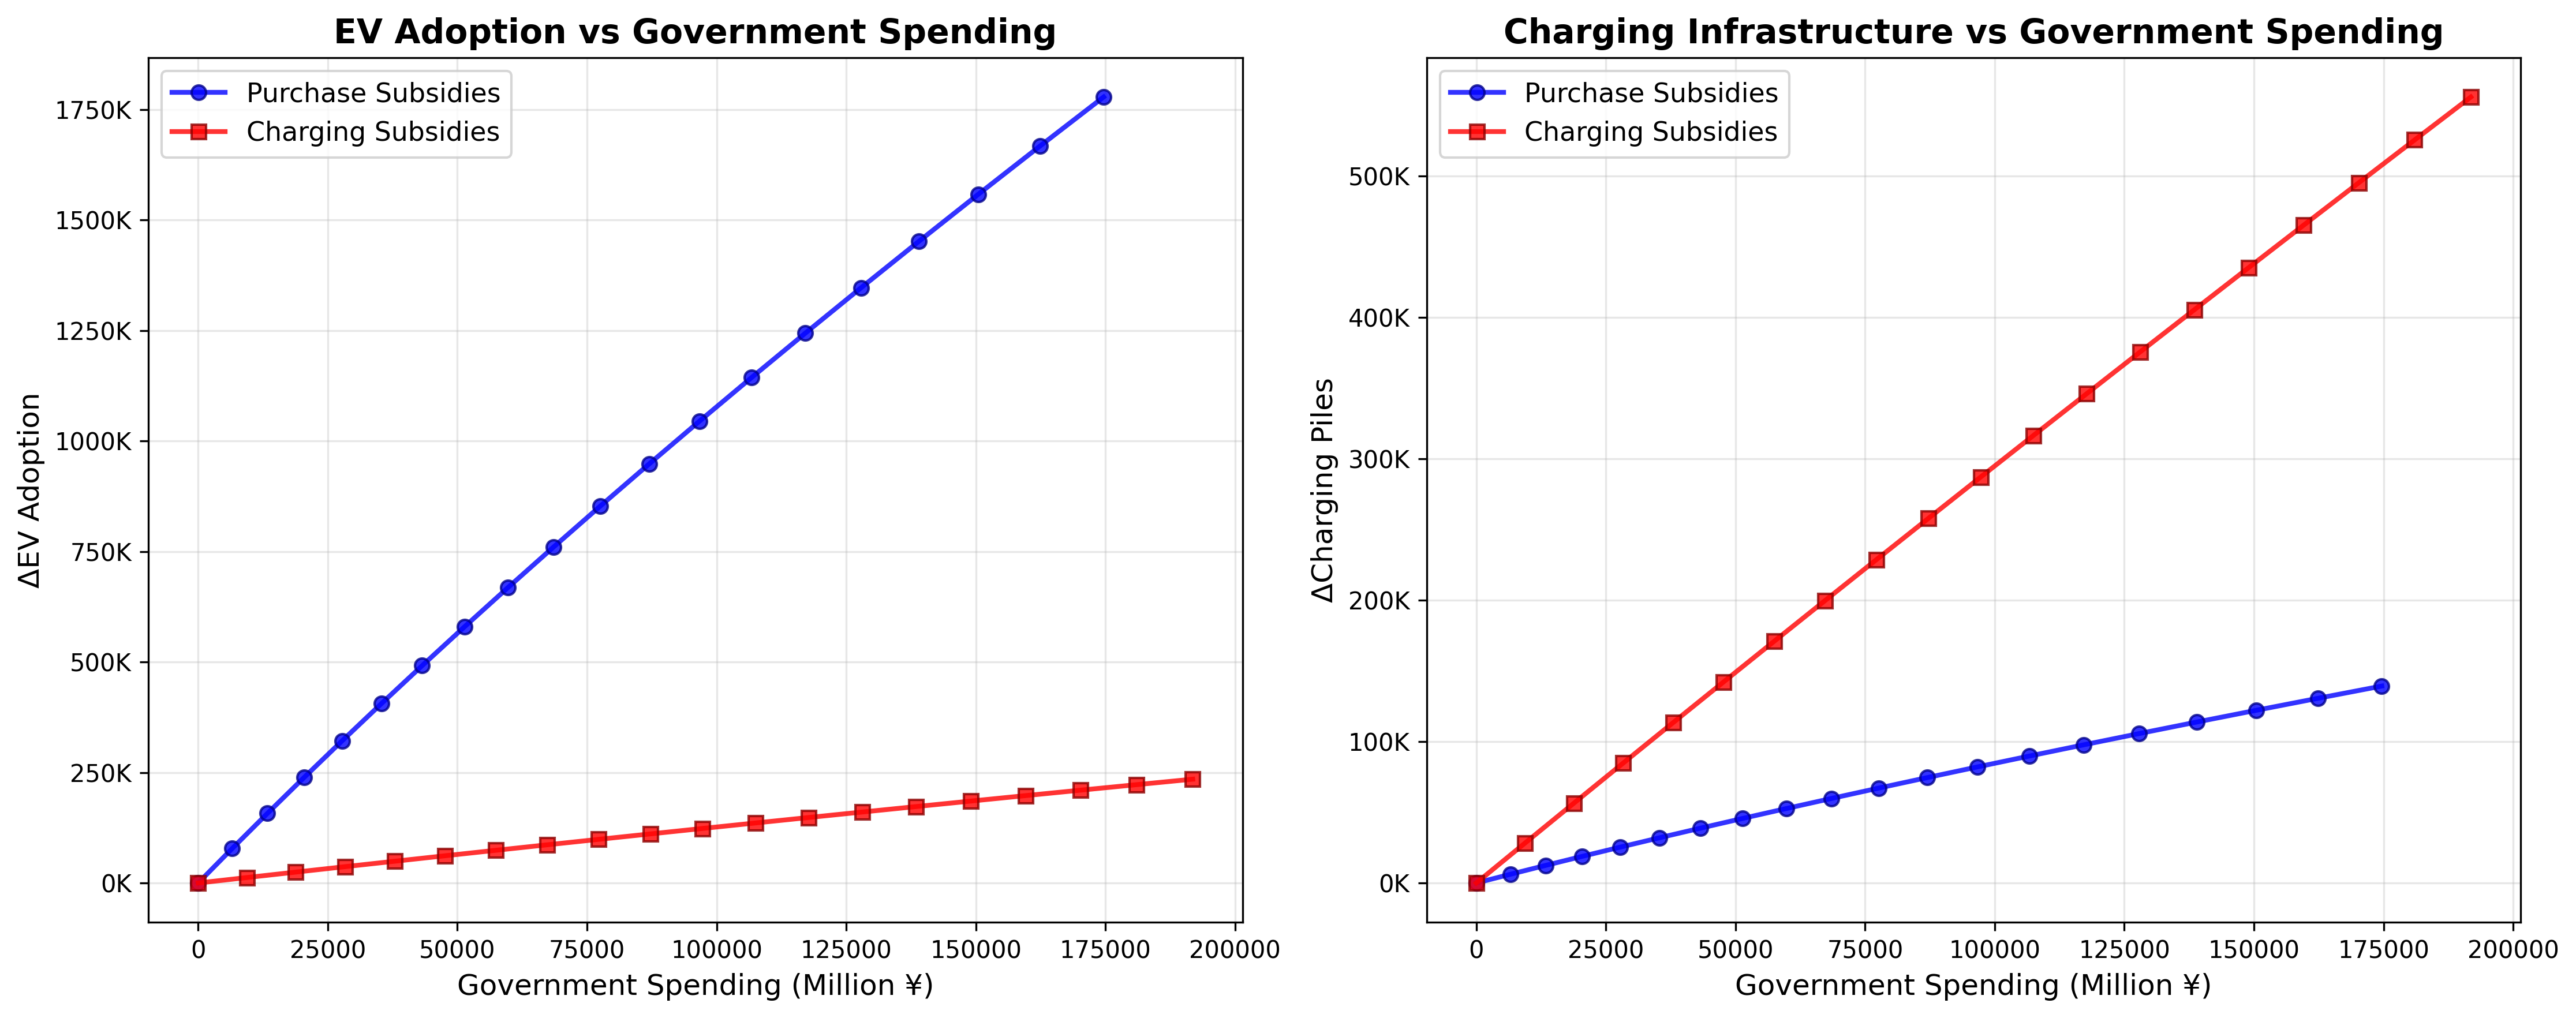
\includegraphics[width=1.0\textwidth]{GraphsTables/policy_counterfactuals_comparison.png}
    \caption{\small Impact of Subsidy Levels on EV Adoption and Charging Infrastructure}
    \label{fig:policy_counterfactuals}
\end{figure}

Figure \ref{fig:policy_counterfactuals} confirms the previous conclusion that indirect network effects are not significant in the Chinese market. 
Purchase subsidies perform better than EVSE subsidies in terms of EV adoption with limited diminishing returns,
whereas the opposite is true for charging infrastructure deployment. 
Relating to previous studies that found charging network expansion exhibiting superior effects than direct subsidies on EV demand, 
the case of the Chinese market could be explained by the relative size of the two sides.
Due to significant amount of policy attention being shifted from EV purchase onto charging infrastructure,
accompanied by the unique hard-quota policies in China, the growth in charging network was actually catching up to EV market size rapidly in the past decade.
Recall that in the results section, insignificant or even reverted network effects had been identified in the analysis on elasticities for many markets,
which was speculated to be caused by the charging network being mature. In fact, a rapidly diminishing return in indirect network effects were documented for the Norwegian market (Springel, 2021).
The Norwegian market, despite having a leading EV adoption rate, still had a relatively nascent EVSE network in the mid 2010s.
The literature generally hypothesizes the initial development of charging network to be crucial, with limited discussions on the later stages when convenience-concerns such as range anxiety no longer applies.
Accounting for the fact that China's EV-piles ratio had dropped below two-to-one, and that the highly elastic vehicle demands, it can be reasonably speculated that the charging network in China on average has been over-developed,
in the sense that consumers have already had access to charging infrastructures to a sufficient levels, making again the price effects from direct incentives more pronounced.


\section{Conclusion}
Incentivizing EV diffusion is crucial for environmental policy, especially for the largest carbon emitter China.
Government efforts in promoting EV adoption and charging infrastructure have shown great successes in China, 
but a comprehensive understanding of the impact of these policies is essential for future policy design.
Motivated by the theoretical framework of two-sided markets, the effectiveness of different subsidies under the presence of indirect network effects remain an empirical question,
and the Chinese market, with its unique significance in global EV growth, is under-studied in this regard.
To address this gap, this study adopts a structural modelling approach accounting for indirect network effects,
to empirically investigates vehicle demand under indirect network effects and policy impacts. 
Specifically, charging infrastructure availability enters for EV demand, while the size of EV base influences charging infrastructure provision.

This study uses data on vehicle sales and public charging piles stock to construct a simultaneous equation model of the two-sided market.
Demand estimation builds on a nested logit model, where consumers first chose products from nests that are defined by fuel types then models to maximize utility.
The charging infrastructure provision model is specified as an equilibrium market outcome where firm entries are based on EV base and entry costs.
The modelling framework is structural in nature, which recovers key model parameters from estimations.
With this framework, I am able to examine the indirect network effects and impact of different subsidies from price elasticities and counterfactual results.

The results and subsequently calculated price-elasticities provide evidence for indirect network effects, 
that the hypothesized two-sidedness of EV and charging providers indeed plays a significant role in shaping market dynamics.
Additionally, two sets of counterfactuals demonstrates that indirect network effects do cause spillover of incentives to the other side of the market, but only to a moderate extent.
Existing policy mix in during the studied period had resulted in 4.7\% more EV sales and 3.3\% more charging piles,
However, from isolated simulations, the efficiency measures in terms of economic impact per million CNY of government spending suggest that,
the current policy mix may not be the most efficient due to limited influence of the indirect network effects.

This study provides insights into the complex interactions between EV demand and charging infrastructure provision in China, 
highlighting the importance of considering both sides of the market in policy design. 
In terms of future works, limitations exist in this study and several improvements can be made to further enrich model implications and policy recommendations.
First, the differentiated product estimation can be extended to incorporate random coefficients, which allows for more flexible substitutional patterns, hence more realistic response to subsidies.
Also, product characteristics can be endogenized to better reflect the impacts of attribute-based subsidies as in Barwick et al. (2024).
Second, strong assumptions are used when defining the charging station entry model, which can be relaxed by introducing elements such as firm heterogeneity and differential impacts from new entries based on spatial data of charging infrastructures.
Lastly, policy information can be enriched and evaluation criteria in counterfactual analyses can made comprehensive to consider product qualities and consumer welfare,
which allows for a more nuanced understanding of policy impacts and better-informed decision-making when chosing across policy instruments.

\end{document}